\section{Evaluation}  \label{sec:evaluation} 
The proposed obstacle aware controller\footnote{Source code: \url{https://github.com/hubernikus/obstacle_aware_damping}} is compared to a baseline, the velocity preserving controller \cite{kronander2015passive}.

\subsection{Qualitative Comparison} \label{sec:qual_comp}
We initially conduct a qualitative analysis of the proposed controller's behavior in various scenarios, as depicted in Figure~\ref{fig:obstacle_aware_damping_comparison}. In each scenario, the agent approaches three obstacles from distinct starting positions. The time step employed is $0.01$ seconds, and the agent's mass matrix is $\matd{M} = \matr{I} m$. The controller is implemented using the following damping values:
$s^{\mathrm{obs}}=~$\qty{200}{s^{-1}},
$s^{\mathrm{f}}=$~\qty{100}{s^{-1}}, and
$s^{\mathrm{c}}=$~\qty{20}{s^{-1}}.
In each scenario, a disturbance (indicated by an arrow) is applied at the same time step. To provide a basis for comparison, the undisturbed trajectory is also displayed alongside the disturbed trajectory.

In the top trajectory, the robot encounters a stand-alone obstacle and experiences a disturbance that pushes it towards the obstacle. With the obstacle-aware controller, the robot adeptly avoids collision and continues moving towards the attractor. In contrast, the baseline controller, which prioritizes velocity conservation, fails to respond effectively and is pushed into the obstacle, resulting in a colliding trajectory.

Moving to the middle trajectory, a disturbance occurs when the agent is positioned between two obstacles. The obstacle-aware controller utilizes the normal vector $\vect n(\vecs \xi)$, as described in Section~\ref{sec:obstacle_repulsion}. However, due to its construction, the magnitude of $\vect n(\vecs \xi)$ diminishes in narrow passages (as seen in \eqref{eq:averaged_normal}), leading to increased damping in all directions, as described in \eqref{eq:leaving_compliance}. As a result, the agent successfully avoids the disturbance using the obstacle-aware controller, while the baseline controller follows a colliding trajectory.

During the bottom trajectory, the repulsive force points away from the obstacle. The obstacle-aware and the velocity-preserving controllers produce nearly identical trajectories due to equal compliance when moving away from an obstacle as defined in \eqref{eq:leaving_compliance}.

We observe the selective damping of disturbances towards the obstacle. The top and middle disturbances are highly damped, while the bottom disturbance is not damped. This feature imparts a natural behavior of moving away from obstacles.
% Furthermore, in Fig.~\ref{fig_run_damped_towards}, one can observe the feature described in Section~\ref{sec:damping_only_toward}, that only damps the disturbance towards the obstacle. The first disturbance is highly damped, while the second is much less. This feature provides a natural behavior of moving away from obstacles, improving the margin of impenetrability. 

\begin{figure}
  \centering
  \centerline{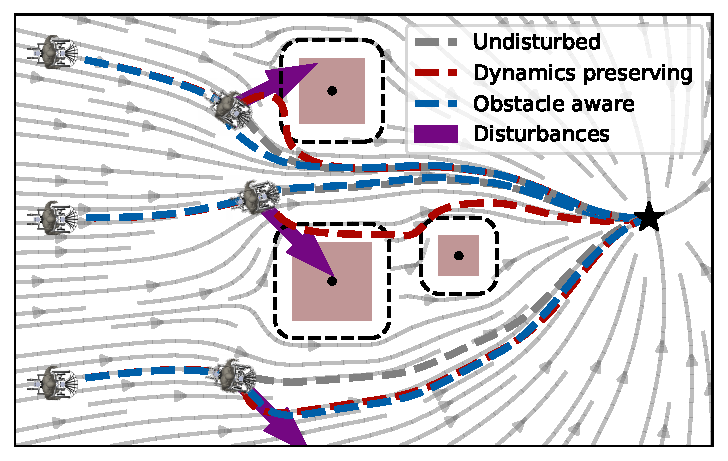
\includegraphics[width=0.95\columnwidth]{figures/multi_obstacle_with_damping.pdf}}
  \caption{
  The desired velocity $\vect f(\vecs \xi)$ is represented in gray and serves as the input for the force controller. The mobile robot, initially positioned at three different locations, navigates safely towards the attractor (black star) even when confronted with external disturbances (purple arrows) while employing the obstacle-aware controller (blue trajectories). In contrast, the baseline controller (red) results in collisions when disturbances occur in close proximity to the robot.
  % The desired velocity $\vect f(\vecs \xi)$ in gray is as input for the force controller. The mobile robot starting from the three positions navigates safely to the attractor (black star) despite the disturbances (red arrows) when using the obstacle-aware controller.   Conversely, the baseline (blue) leads to collision when the disturbance happens close to the robot.
  }
  \label{fig:obstacle_aware_damping_comparison}
\end{figure}

\subsection{Noise Analysis}
In practical robotic applications, real controllers are inevitably exposed to noise and unexpected disturbances, arising from sensor inaccuracies, environmental factors, or other external perturbations. A high-quality controller is able to effectively reject such disturbances while simultaneously achieving its control objectives, such as collision avoidance and trajectory tracking.

This section investigates the impact of noise disturbances on a simulated agent with an identity mass matrix $\matd M = \matr I m$. The discrete time step is set to $\Delta t = $\qty{0.2}{s}. Additionally, the damping values are configured as follows: 
$s^{\mathrm{obs}}=$~\qty{50}{s^{-1}},
$s^{\mathrm{f}}=$~\qty{40}{s^{-1]}}, and
$s^{\mathrm{c}}=$~\qty{5}{s^{-1}}.
%to follow the linear velocity field of  the form $\vect f(\vecs \xi) = (\vecs \xi^a -  \vecs \xi)$,nd the velocity is capped at a magnitude of \qty{1}{m/s}.  The controllers are compared by analyzing the minimal distance to the surface along a trajectory $ \min_t \| \vecs \xi_t - \vecs \xi^b \| $, see \eqref{eq:distance_function}.
The robot's objective is to follow a linear velocity field of the form $\vect f(\vecs \xi) = (\vecs \xi^a - \vecs \xi)$ with a velocity cap of \qty{1}{m/s}.
To evaluate the controller's performance, a comparative analysis is conducted by assessing the minimal distance to the surface along the trajectory, denoted as $ \min_t \| \vecs \xi_t - \vecs \xi^b \| $, with the boundary point $\vecs \xi_b$ described in \eqref{eq:distance_function}. 

\subsubsection{Velocity Noise Resistance}
In the initial evaluation, we introduce normally distributed noise with a mean of zero into the agent's velocity $\dot{\vecs{ \xi}}$ before computing the control force (Fig.~\ref{fig:velocity_noise}). 

Remarkably, the obstacle-aware controller effectively rejects the noise impacting the velocity, even as the noise variance increases. However, it is essential to note that the closest distance during the trajectory diminishes with higher noise variance. On the contrary, the velocity-following controller's mean distance falls below zero already at a velocity noise variance of $\qty{0.5}{m/s}$, indicating that a substantial number of trajectories collide with at least one obstacle.

Furthermore, in the absence of noise, the obstacle-aware controller maintains a higher minimal distance along the trajectory. This effect results from the higher damping applied towards the obstacle, enabling more precise tracking of the curvature guiding the velocity around the obstacle.

\begin{figure}
    \centering
    \begin{subfigure}{\columnwidth}
      \centerline{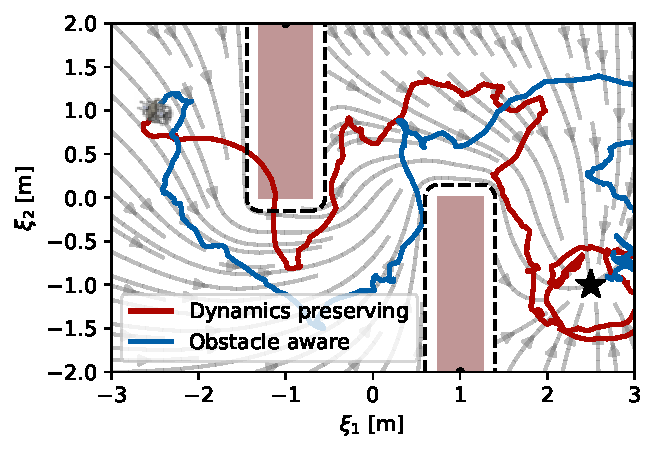
\includegraphics[width=\textwidth]{figures/trajectory_velocity_noise}}
      \caption{Trajectories with a standard deviation of the velocity-noise of 1.0 m/s.}
      \label{fig:trajectory_velocity_noise}
    \end{subfigure}
    \begin{subfigure}{\columnwidth}
    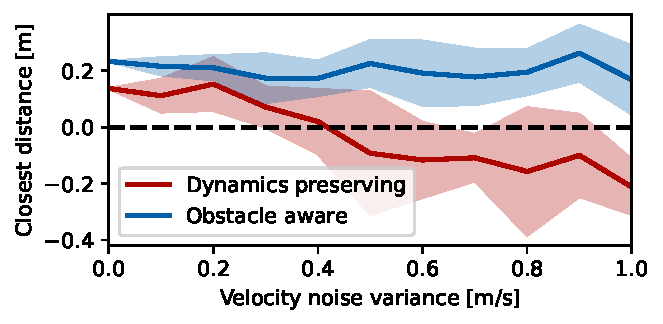
\includegraphics[width=\textwidth]{figures/comparison_velocity_noise}
      \caption{The mean and variance (shaded) of the closest distances over 10 epochs.}
      \label{fig:comparison_velocity_noise}
    \end{subfigure}
	\caption{The agent navigates between two elongated obstacles (a) towards the attractor (black star). The agent's velocity is subjected to white noise, with a mean of zero, and noise variances between \qty{0.0}{m/s} and \qty{1.0}{m/s}. The robot initiates its trajectory from the starting position $\vecs \xi_0 = [-2.5, 1.0]^T$, with an initial velocity of zero. It aims to reach the attractor located at $\vecs \xi^a = [2.5, -1.0]^T$.}
\label{fig:velocity_noise}
\end{figure}

\subsubsection{Position Noise Resistance} \label{sec:position_noise}
In the second experiment, normally distributed noise with a mean of zero is added to the position $\vecs{ \xi}$ (Fig.~\ref{fig:position_noise}). 

The obstacle-aware controller maintains a greater distance to the surface even when no noise is present, while the velocity-preserving controller already exhibits collisions. As a result, the obstacle-aware creates trajectories with the mean of the distance above zero for standard deviations of the position noise smaller than \qty{0.023}{m}. Conversely, for the velocity-preserving controller, the mean distance to the surface is below zero for all experiment runs, indicating collisions.
It is important to note that this difference is attributed to the buffer mechanism inherent in the obstacle-aware controller. Despite a similar decrease in distance for both controllers, the obstacle-aware controller effectively prevents collisions due to its higher impedance towards the obstacles.

Moreover, the velocity-preserving controller exhibits a higher variance of distance, likely stemming from its lower damping, causing it to adapt more slowly to new velocities after being displaced by the noise. Consequently, this behavior leads to more random variations in velocity and trajectory.

\begin{figure}
    \centering
    \begin{subfigure}{\columnwidth}
      \centerline{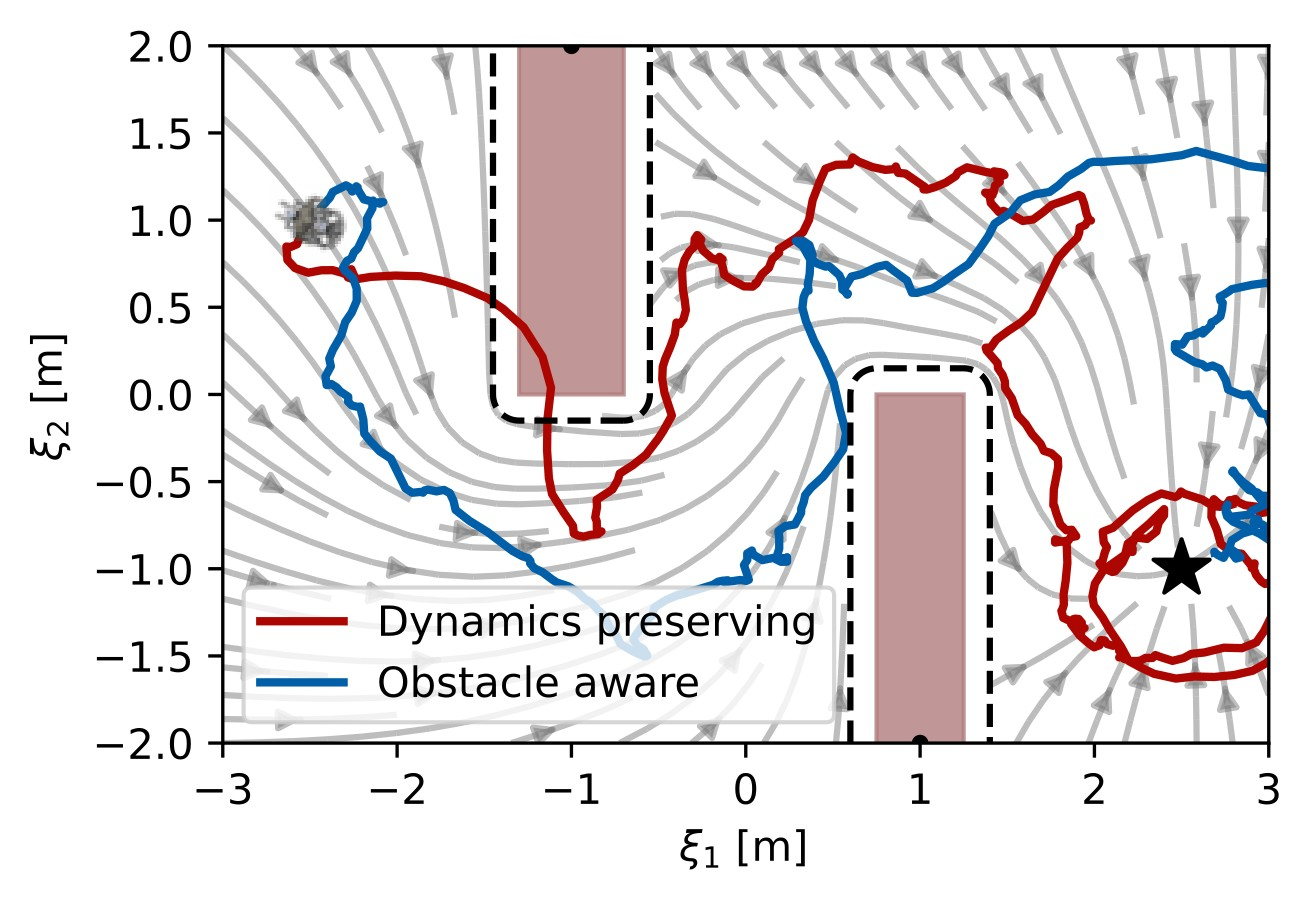
\includegraphics[width=\textwidth]{figures/trajectory_position_noise}}
      \caption{Trajectories with a standard deviation of the position-noise of 0.0 m.}
      \label{fig:trajectory_position_noise}
    \end{subfigure}
    \begin{subfigure}{\columnwidth}
    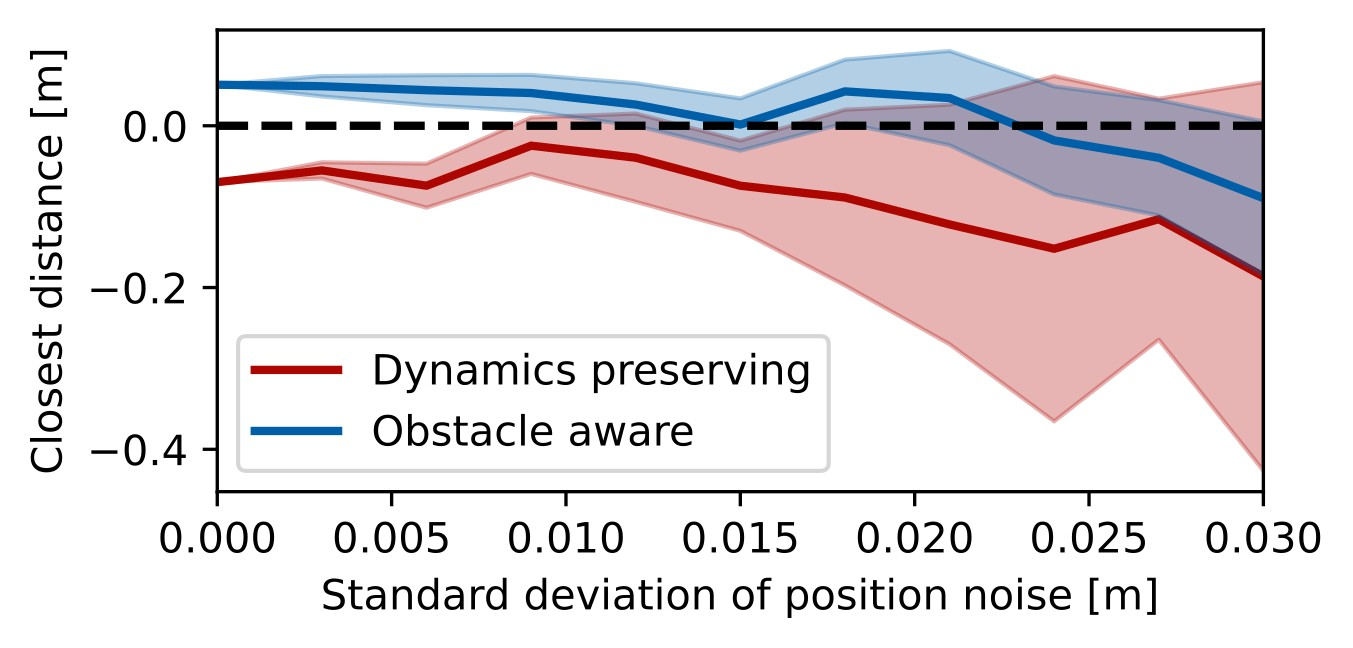
\includegraphics[width=\textwidth]{figures/comparison_position_noise}
      \caption{Closest distances concerning different noise levels over 10 epochs.}
      \label{fig:comparison_position_noise}
    \end{subfigure}
	\caption{
 The agent is navigating towards the attractor (black star) between two concave obstacles (a) while being subjected to white noise in its position. The position noise has a mean of zero, and various noise variances ranging between \qty{0.0}{m} and \qty{0.03}{m}. The robot starts at position $\vecs \xi_0 = [-2.5, -1.0]^T$, and the attractor is set to $\vecs \xi^a = [2.5, 1.0]^T$.
 }
\label{fig:position_noise}
\end{figure}


\subsection{Obstacle Aware Passivity Using a Robot Arm}
The obstacle-aware passivity controller was implemented to guide a 7-degree-of-freedom robot arm (Panda from Franka Emika) while effectively avoiding collisions. 

The joint torque is computed using inverse kinematics:
\begin{equation}
	\vecs \tau_q = \matr J^{\dag}(\vect q) 
	\begin{bmatrix} \matd D(\vecs \xi) \left( \vect f(\vecs \xi) - \dot{\vecs \xi} \right) \\  p^\alpha (\vecs \alpha - \vecs \alpha^a) \end{bmatrix}
\end{equation}
where $\matr J^{\dag}$ represents the Moore-Penrose pseudo inverse of the Jacobian matrix, and $\vecs \alpha$ and $\vecs \alpha^a$ denote the end effector's orientation and the desired orientation, respectively. The angular damping parameter is chosen as $p^\alpha = 5.5$.
The desired orientation $\vecs \alpha^a$ is pointing downward with a quaternion value of $(w, x, y, z) = (0, 1, 0, 0)$. For the subtraction, we use quaternion representation to avoid singularities, but for the evaluation of the torque from the angular offset angle-axis representation of the orientation is used.
% using the Moore-Penrose pseudo inverse of the Jacobian $\matr J^{\dag} = \matr J^T (\matr J \matr J^T)^{-1}$. The angle $\vecs \alpha$ describes the end effector orientation, and the desired orientation $\vecs \alpha^a$ is pointing downward with a quaternion value of $(w, x, y, z) = (0, 1, 0, 0)$. For the subtraction, we use quaternion representation to avoid singularities, but for the evaluation of the torque from the angular offset angle-axis representation of the orientation is used.

The angular damping is chosen as $p^\alpha = 5.5$.
The damping values are set as
$s^{\mathrm{obs}}=$~\qty{160}{s^{-1}},
$s^{\mathrm{f}}=$~\qty{64}{s^{-1]}}, and
$s^{\mathrm{c}}=$~\qty{16}{s^{-1}}.

The robot start position is approximately at $\vecs \xi_0 = [0.3\mathrm{m}, 0.4\mathrm{m}, 0.3\mathrm{m},]^T$ and the attractor is at position $\vecs \xi^a = [0.26 \mathrm{m}, -0.53\mathrm{m}, 0.33\mathrm{m}]^T$.
The robot encounters a single squared box with axes length \qty{0.16}{m} and a margin of \qty{0.12}{m}, placed approximately at the center between the start and attractor positions. The precise location of the box is tracked in real-time using a marker-based vision system (Optitrack). As the robot passes by the box, it is disturbed by a strong push $\vecs t^e$ towards the box. The experiment is repeated ten times for both controllers, as well as for the undisturbed motion.
% The motion is guided by the dynamical system in the presence of a single squared box with axes length \qty{0.16}{m}, and a margin of \qty{0.12}{m}. The box is placed approximately at the center of the start and attractor, but the precise location  is obtained at each time step using a marker based vision system (Optitrack).  While passing the box, the robot is disturbed by a strong push $\vecs t_e$ towards the box. The sequence is repeated 10 times for both controllers, as well as for the undisturbed motion.

% From the experimental results in Figure~\ref{fig:evaluation_on_robot_arm}, it is observed that using the obstacle ware controller, the robot is able to stay on average \qty{0.15}{m} away from the obstacle surface. While for the velocity preserving controller, the mean distance is below \qty{0.05}{m}, and many trajectories collide with the box. 
% This results from a much weaker control force of the obstacle-aware controller. Which has a high peak as soon as the disturbance occurs, at around \qty{1.45}{s}. Conversely, for the velocity preserving trajectory, no such high peak occurs, and the controller only acts when the robot is almost colliding. In fact, the obstacle-aware controller already shows high forces before the disturbance, this additionally results in improved tracking of the avoidance trajectory as we've seen in Section~\ref{sec:position_noise}.
The experimental results in Figure~\ref{fig:evaluation_on_robot_arm} demonstrate that the obstacle-aware controller allows the robot to maintain an average distance of \qty{0.15}{m} away from the obstacle surface. In contrast, the velocity-preserving controller results in a mean distance below \qty{0.05}{m}, and numerous trajectories lead to collisions with the box. On average, the robot passes further away from the obstacle using the obstacle-aware controller and exhibits higher forces, Table~\ref{tab:evaluation_on_robot_arm}.

\begin{table}[htb]
% Distance [NoDist]: 0.1672703839  \pm 0.009033828534378131
% Distance [PassiveDS]: 0.018012260429208955  \pm 0.02613021511175264
% Distance [Aware]: 0.10564614093567434  \pm 0.02136799916777507
% No-Interaction Force: 2.8572200673080523 \pm 0.36821047478539665 
% No-Damping Force: 3.5782840941712544 \pm 0.23762587158014598 
% Obstacle-Aware Force: 4.1208857008362125 \pm 0.25191997294727264 
    \centering
    \begin{tabular}{|l|c|c|c|} \hline
        & Obstacle & Velocity & Undisturbed \\ \hline
         Closest Distance [mm] &  105 $\pm$ 21 & 18 $\pm$ 21 & 167 $\pm$ 9 \\ \hline
         Maximum Force [N] & 4.12 $\pm$ 0.25 & 3.58 $\pm$ 0.24 & 2.86 $\pm$ 0.37  \\ \hline 
    \end{tabular}
    \caption{The mean and standard deviation of the closest distance and maximum force over the 10 epochs.}
    \label{tab:evaluation_on_robot_arm}
\end{table}

This outcome is attributed to the obstacle-aware controller's stronger control force, with a high peak occurring around \qty{1.45}{s} when the disturbance is encountered. In contrast, the velocity-preserving controller only reacts when the robot is almost colliding, leading to a delayed response. Additionally, the obstacle-aware controller exhibits higher forces even before the disturbance, which contributes to improved tracking of the avoidance trajectory, as observed in Section~\ref{sec:position_noise}. These findings affirm the superior collision avoidance capabilities and tracking performance of the obstacle-aware passivity controller in real-world robot arm scenarios.


\begin{figure}
    \centering
   \begin{subfigure}{\columnwidth}
    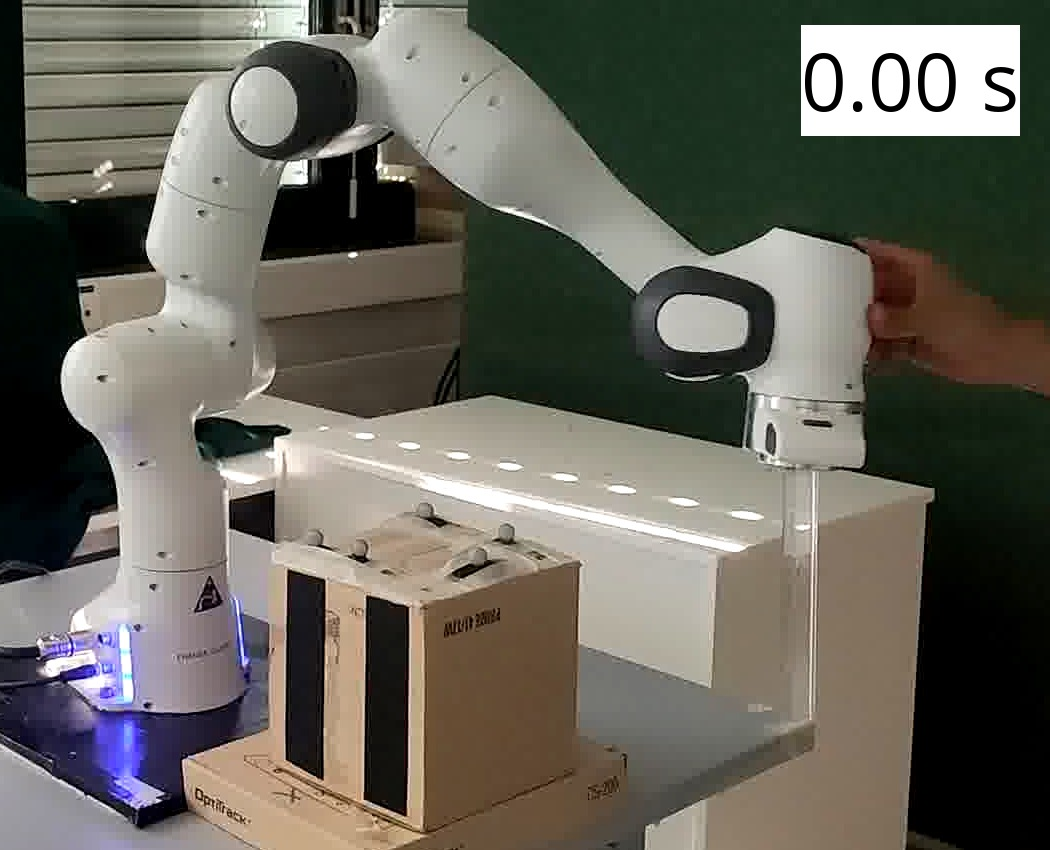
\includegraphics[width=0.49\textwidth]{figures/franka_sequence/franka_obstacle_aware016}\hfill%
    % 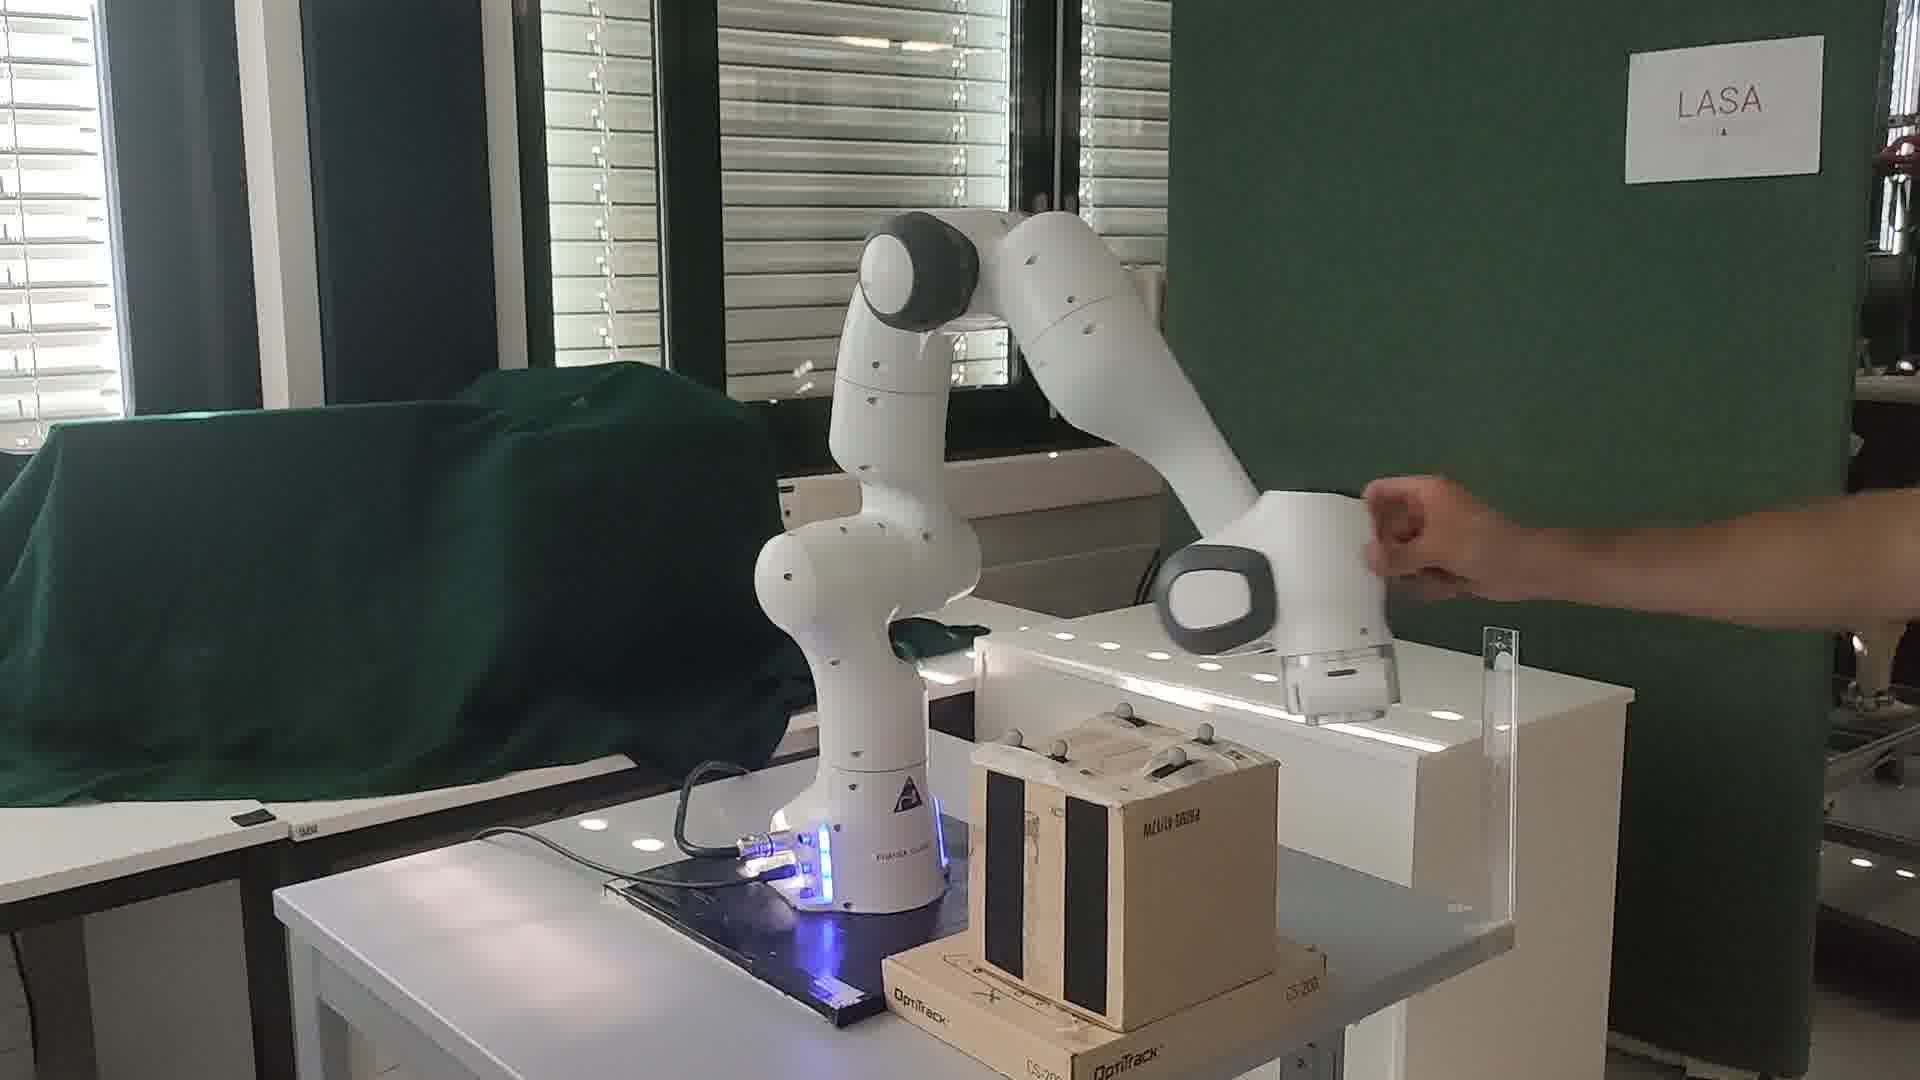
\includegraphics[width=0.33\textwidth]{figures/franka_sequence/franka_obstacle_aware018}\hfill%
    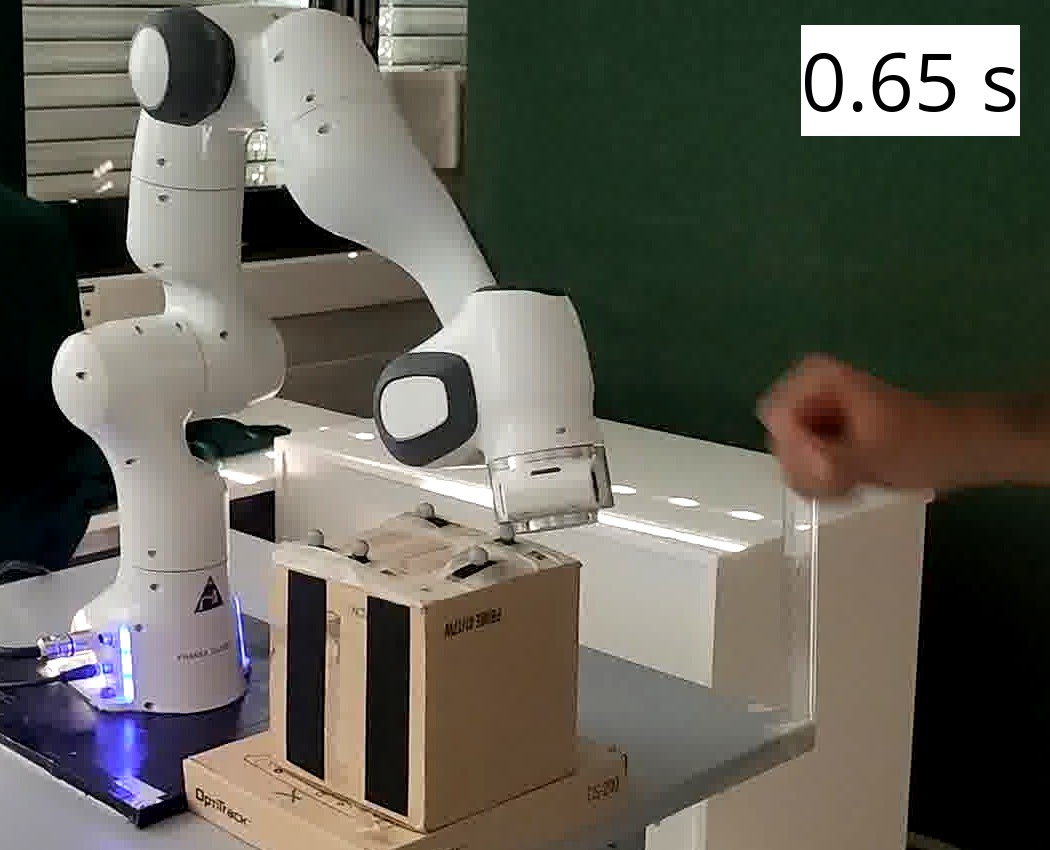
\includegraphics[width=0.49\textwidth]{figures/franka_sequence/franka_obstacle_aware020}
      \caption{Obstacle-aware controller rejects repulsion and avoids collision}
      \label{fig:franka_sequence_obstacle_aware}
    \end{subfigure}
	\begin{subfigure}{\columnwidth}
    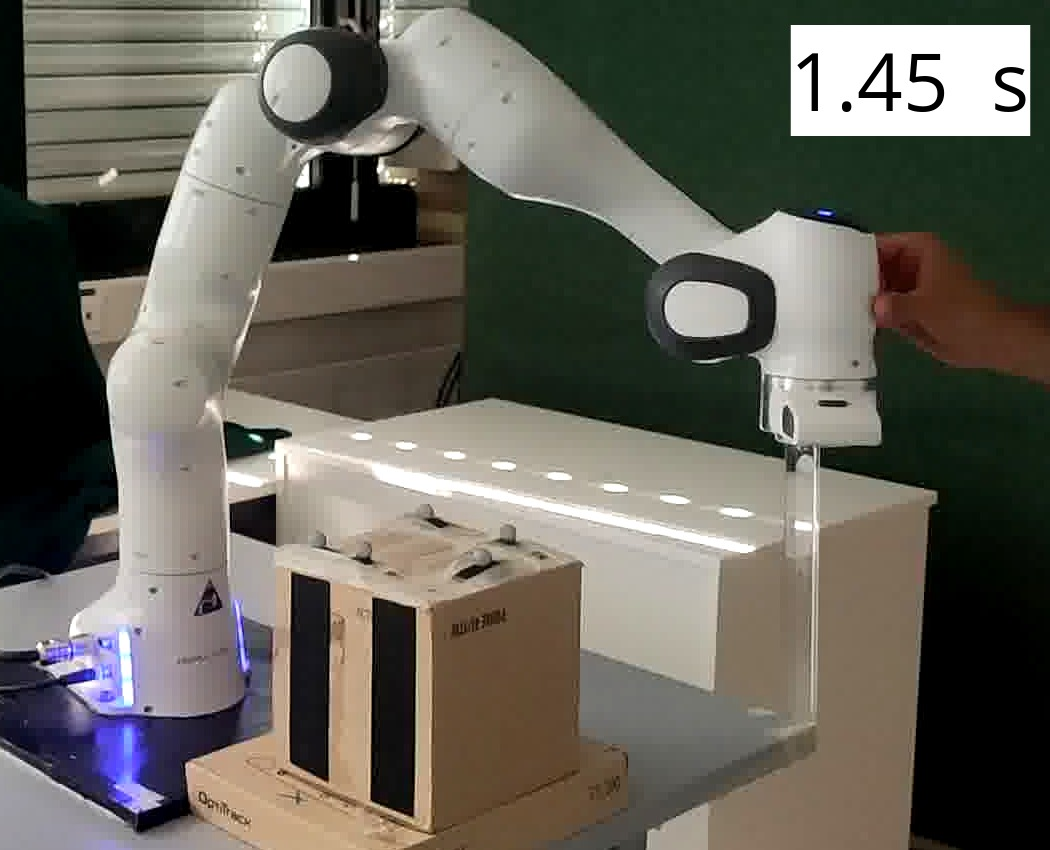
\includegraphics[width=0.49\textwidth]{figures/franka_sequence/franka_velocity_conserving021}\hfill%
    % 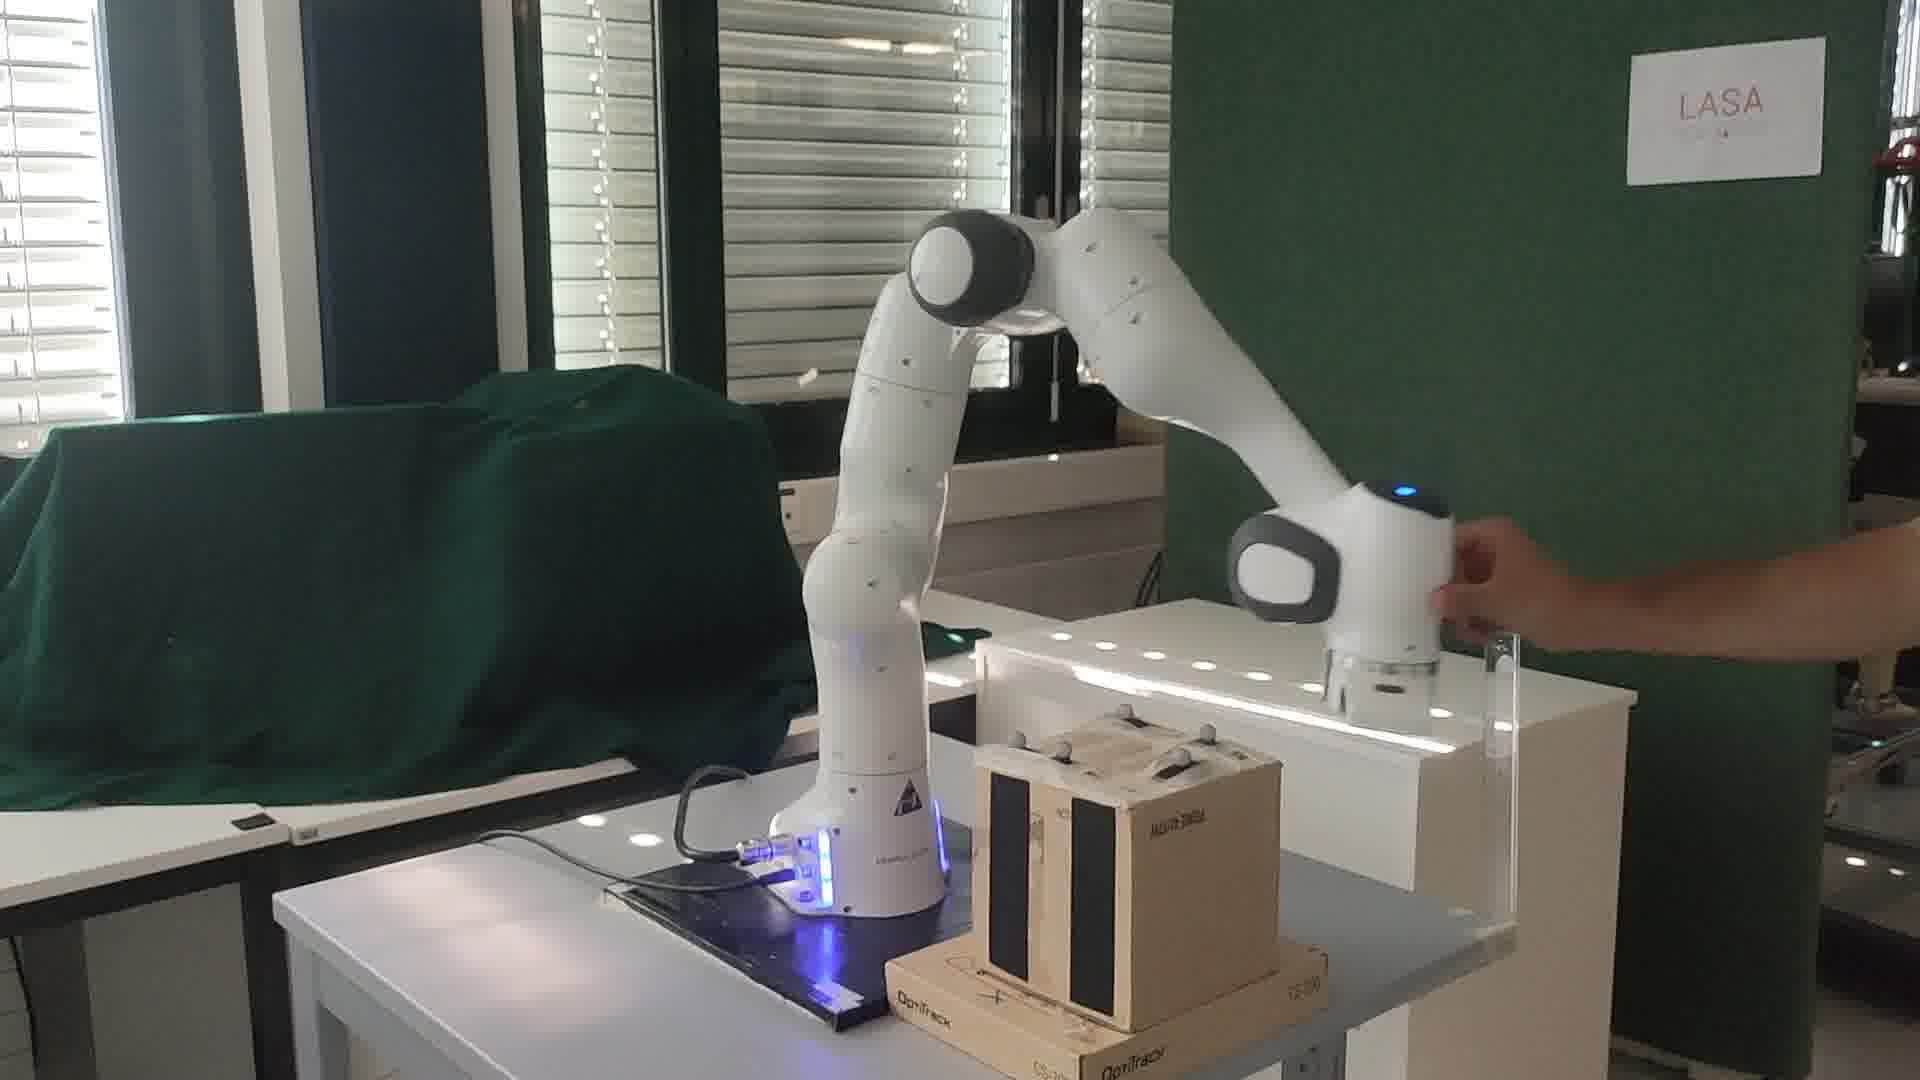
\includegraphics[width=-1.33\textwidth]{figures/franka_sequence/franka_velocity_conserving023}\hfill%
    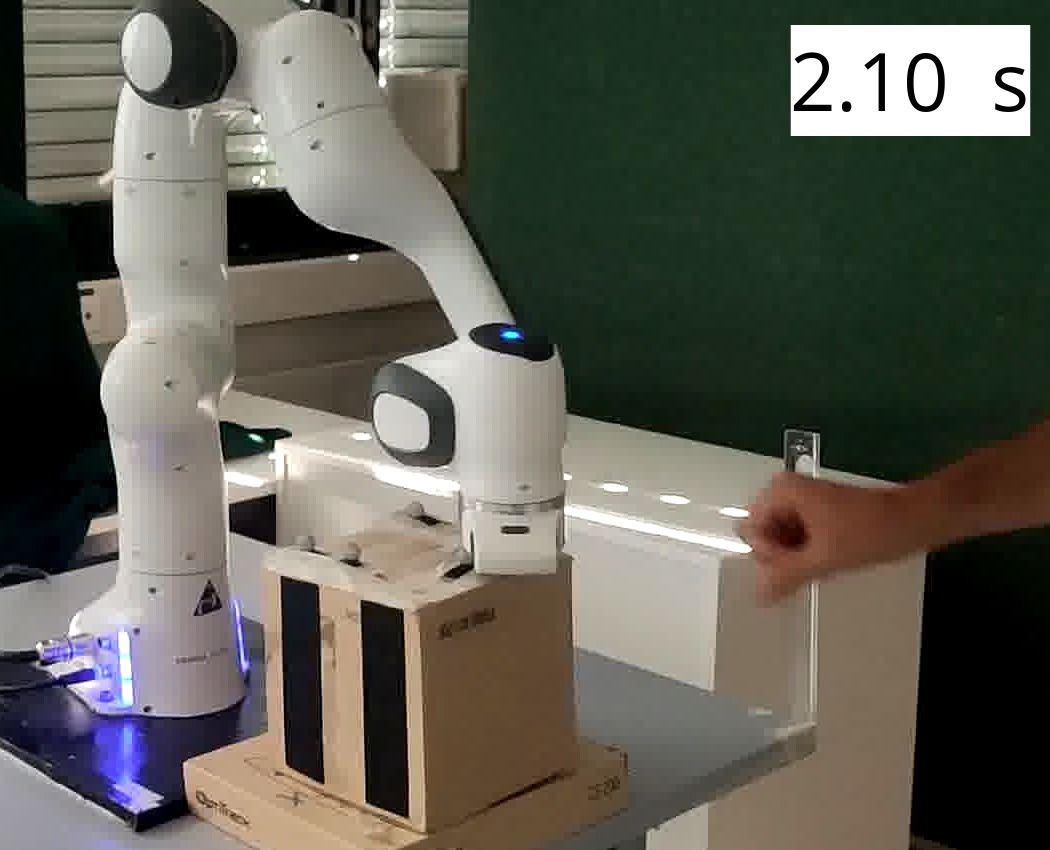
\includegraphics[width=0.49\textwidth]{figures/franka_sequence/franka_velocity_conserving025}\hfill%
      \caption{Velocity preserving controller leads to collision with obstacle}
      \label{fig:franka_sequence_obstacle_aware}
    \end{subfigure}
%    \caption{Comparison of the two control methods}
%    \label{fig:evaluation_on_robot_arm}
% \end{figure}
% \begin{figure}
%     \centering
    \begin{subfigure}{\columnwidth}
      \centerline{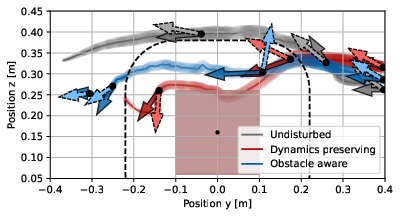
\includegraphics[width=\textwidth]{figures/robot_arm_trajectory_xyz}}
      \caption{The two control methods compared with the undisturbed trajectory. The wider line indicates a higher x-value. The darker arrow is the actual, and the brighter is the desired velocity.}
      \label{fig:robot_arm_trajectory_xyz}
    \end{subfigure}
    \begin{subfigure}{\columnwidth}
		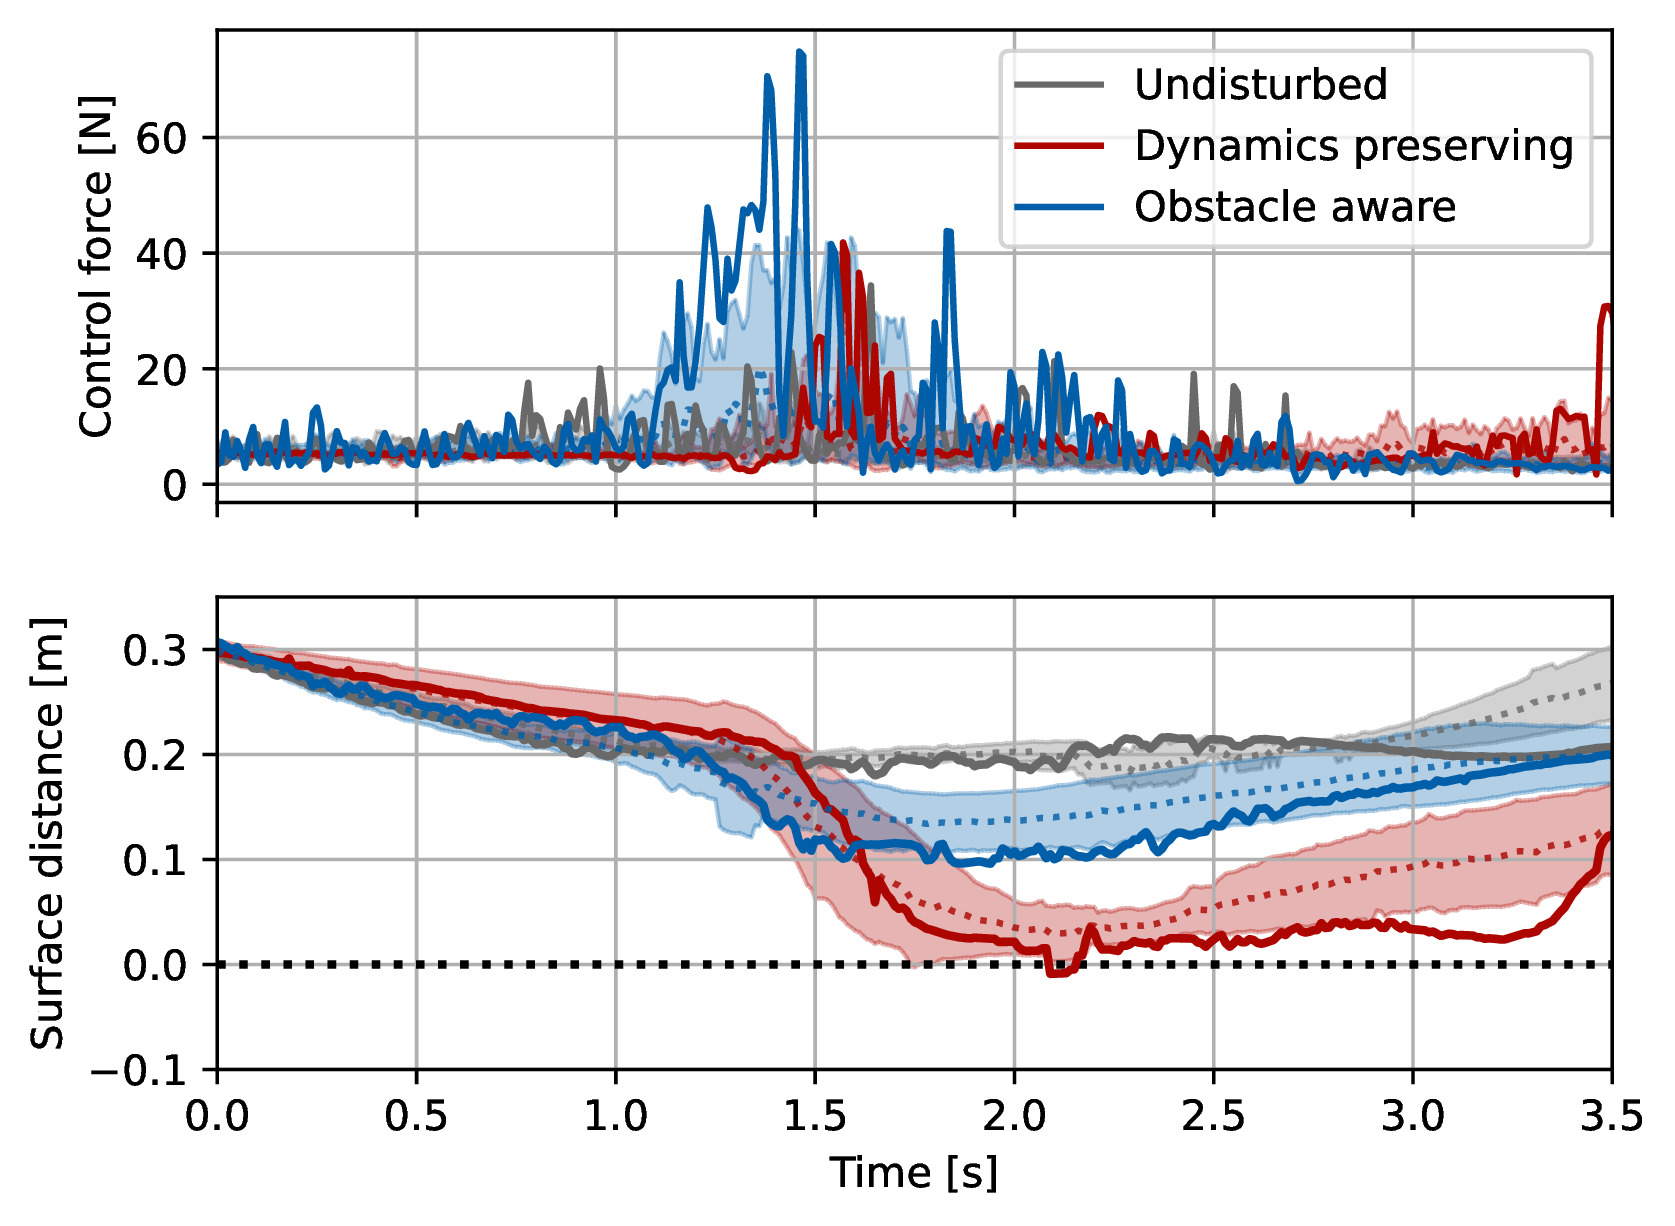
\includegraphics[width=\textwidth]{figures/trajectory_comparison_force_and_distance}
      \caption{The specific trajectory is represented by a full line, while the average (dashed line) and variance (shaded area) are evaluated over 10.  Regarding the control force, both the mean and variance are evaluated in the logarithmic space.}
      \label{fig:trajectory_comparison_force_and_distance}
    \end{subfigure}
	\caption{
The robot arm, guided by the obstacle-aware passive controller, effectively avoids the disturbance towards the obstacle while maintaining a margin of 0.16m around the obstacle. The experiment was repeated 10 times with a similar disturbance applied to the robot arm in each run.
 }  
    \label{fig:evaluation_on_robot_arm}
\end{figure}

\section{Discussion}
The simulated robot demonstrates promising results, exhibiting good tracking performance, compliance in the direction perpendicular to the motion, and effective damping of disturbances towards obstacles. The controller performs similarly to the approach presented in \cite{kronander2015passive} when away from obstacles. However, as the robot approaches an obstacle, the control becomes more damped to avoid collisions without compromising its tracking capabilities. This characteristic renders the proposed controller suitable for achieving both precise tracking and obstacle avoidance safety.

In the simulation, the robot was able to repulse disturbances in velocity and in position. This allowed the smooth deployment of the algorithms on the real robot arm. Where the proposed controller has been successful in avoiding collision while still remaining compliant.

\subsection{Applicability and Theoretical Analysis}
It is worth noting that the theoretical analysis from Theorem~\ref{theorem:passivity} indicates passivity for any velocity-bounded, uniquely damped system. Consequently, controllers like the damping-based approach in \cite{kronander2015passive} no longer require an energy tank. Conversely, if the impedance controller features a proportional term $\mathcal{K}$, the adaptive proportional term may induce instabilities, even for a stable desired velocity, as highlighted in \cite{ferraguti2013tank, kronander2016stability}. Careful consideration of the controller design and stability analysis is necessary to ensure robust and safe performance in practical applications.